%# -*- coding: utf-8-unix -*-
%======================================================================
% qbook.tex for Qbook Template
%======================================================================
% 双面打印
\documentclass{qbook}
\addbibresource{bib/qbook.bib}  % 导入参考文献数据库
\begin{document}
\pagestyle{empty}
%# -*- coding: utf-8-unix -*-
\thispagestyle{empty}
\begin{tikzpicture}[overlay,remember picture,font=\sffamily\bfseries]
\draw[ultra thick,c4,name path=big arc] ([xshift=-2mm]current page.north) arc(150:285:11)
coordinate[pos=0.225] (x0);
\begin{scope}
\clip ([xshift=-2mm]current page.north) arc(150:285:11) --(current page.north
east);
\fill[c4!50,opacity=0.25] ([xshift=4.55cm]x0) circle (4.55);
\fill[c4!50,opacity=0.25] ([xshift=3.4cm]x0) circle (3.4);
\fill[c4!50,opacity=0.25] ([xshift=2.25cm]x0) circle (2.25);
\draw[ultra thick,c4!50] (x0) arc(-90:30:6.5);
\draw[ultra thick,c4] (x0) arc(90:-30:8.75);
\draw[ultra thick,c4!50,name path=arc1] (x0) arc(90:-90:4.675);
\draw[ultra thick,c4!50] (x0) arc(90:-90:2.875);
\path[name intersections={of=big arc and arc1,by=x1}];
\draw[ultra thick,c4,name path=arc2] (x1) arc(135:-20:4.75);
\draw[ultra thick,c4!50] (x1) arc(135:-20:8.75);
\path[name intersections={of=big arc and arc2,by={aux,x2}}];
\draw[ultra thick,c4!50] (x2) arc(180:50:2.25);
\end{scope} 
\path[decoration={text along path,text color=c4,
	raise = -2.8ex,
	text  along path,
	text = {|\sffamily\bfseries|\today},
	text align = center,
},
decorate
] ([xshift=-2mm]current page.north) arc(150:245:11);
%
\begin{scope}
\path[clip,postaction={fill=c3}]
([xshift=2cm,yshift=-8cm]current page.center) rectangle ++ (4.2,7.7);
\fill[c2] ([xshift=0.5cm,yshift=-8cm]current page.center)
([xshift=0.5cm,yshift=-8cm]current page.center)  arc(180:60:2)
|- ++ (-3,6) --cycle;
\draw[ultra thick,c4] ([xshift=-1.5cm,yshift=-8cm]current page.center) 
arc(180:0:2);
\draw[ultra thick,c4] ([xshift=0.5cm,yshift=-8cm]current page.center) 
arc(180:0:2);
\draw[ultra thick,c4] ([xshift=2.5cm,yshift=-8cm]current page.center) 
arc(180:0:2);
\draw[ultra thick,c4] ([xshift=4.5cm,yshift=-8cm]current page.center) 
arc(180:0:2);
% \fill[red] ([xshift=2.5cm,yshift=-8cm]current page.center) +(60:2) circle(1.5mm);
% \node[text=c5!80!black] at ([xshift=4.7cm,yshift=-5.2cm]current page.center) {$\rho:=\dfrac{1+\sqrt{-3}}{2}$};
\end{scope}
%
\fill[c1] ([xshift=2cm,yshift=-8cm]current page.center) rectangle ++ (-13.7,7.7);
\node[text=white,anchor=east,scale=4,inner sep=0pt] at
([xshift=1.8cm,yshift=-3cm]current page.center) {西浦博士生攻略};
\node[text=white,anchor=east,scale=2,inner sep=0pt] at
([xshift=1.8cm,yshift=-5.5cm]current page.center) {PGR Society 社团\quad 制作};
\node[text=white,anchor=east,scale=2,inner sep=0pt] at
([xshift=1.8cm,yshift=-6.5cm]current page.center) {主编\quad 吴开};
\end{tikzpicture}  % 载入封面
\begin{center}
	\Large{\sffamily\bfseries\heiti Version 0.0.1} \\ \vspace{2em}
	\Large{\sffamily\bfseries\heiti 编译日期: \today} \\ \vspace{1em}
\end{center} 
\vfill
\vspace{30em}
\begin{tabular*}{\textwidth}{ccc}
	\includegraphics{figure/by-nc.eps}
	& \begin{minipage}[b]{0.6\textwidth}
		\small\sffamily
		本作品采用知识共享 署名-非商业性使用 4.0 国际 许可协议进行许可. 访问\url{http://creativecommons.org/licenses/by-nc/4.0/  }查看该许可协议.
	\end{minipage}
\end{tabular*}  
\thispagestyle{empty}
\frontmatter  % 对前言和概览用罗马数字作为页码
\pagestyle{empty}

\begin{pre}
	\thispagestyle{empty}
	\begin{center}
		{\kaishu{人在春风和气中}}
	\end{center}

\vspace*{5\baselineskip}
\centerline{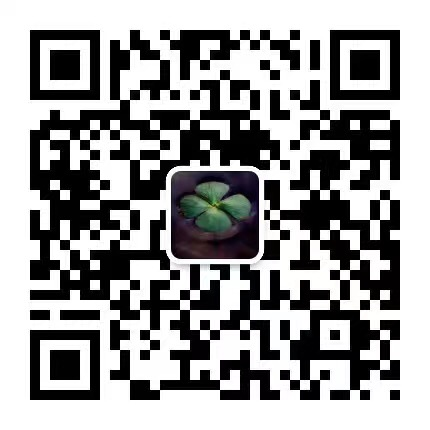
\includegraphics[scale=0.6]{example/gzh.jpg}}
\centerline{\fontsize{26pt}{26pt} 微信公众号}
\end{pre}
\pagestyle{empty}
\tableofcontents
% \cleardoublepage
% %# -*- coding: utf-8-unix -*-
\begin{overview}
\thispagestyle{empty}

必修课程

APR

Liverpool Life 会议记录

助教

监考

PGR Society 研究生社团

福利:
会议经费
免费办公用品
免费打印
体育馆代金券
茶和咖啡
Liverpool 免费高级Zoom账户 
\url{https://liverpool.service-now.com/sp?id=kb_article&sysparm_article=KB0011854}

Liverpool 免费 Office365
\url{https://liverpool.service-now.com/sp?id=kb_article&sysparm_article=KB0010032}

Liverpool 免费 1T Onedrive 云盘 网页使用
\url{https://liverpool.service-now.com/sp?id=kb_article&sysparm_article=KB0011362}

Liverpool 免费 1T Onedrive 云盘 本地备份同步
\url{https://support.microsoft.com/zh-cn/office/%E4%BD%BF%E7%94%A8-onedrive-%E8%BF%9B%E8%A1%8C%E5%90%8C%E6%AD%A5-bb89981b-e382-4969-b8fd-d413a90b6db3}

其他Liverpool免费软件
\url{https://www.liverpool.ac.uk/it/software/software-downloads/}

Liverpool软件序列号
\url{https://www.liverpool.ac.uk/it/software/licencecodes/}

其他攻略:
如何远程访问校内电脑
西浦虚拟机

避坑:
学校的网盘不能用于分享文件


\end{overview}
 
\mainmatter	  % 对正文用阿拉伯数字作为页码
%======================================================================
% 正文内容
\pagestyle{fancy}
\setcounter{page}{0}
%# -*- coding: utf-8-unix -*-
%%==================================================
\chapter{这些必须得做,不然毕不了业}
\label{must-do}

非常重要,一定要认真准备

\section{必修课程}

\section{Liverpool Life 会议记录}

\section{APR}


%# -*- coding: utf-8-unix -*-
%%==================================================

\chapter{这些必须得看,不看吃大亏}
\label{fuli}

\section{会议经费}
\section{免费办公用品}
\section{免费打印}
\section{体育馆代金券}
\section{茶和咖啡}
\section{利物浦账号自带福利}
\begin{itemize}
    \item Liverpool 免费高级Zoom账户:\url{https://liverpool.service-now.com/sp?id=kb_article&sysparm_article=KB0011854}
    \item Liverpool 免费 Office365:\url{https://liverpool.service-now.com/sp?id=kb_article&sysparm_article=KB0010032}
    \item Liverpool 免费 1T Onedrive 云盘 网页使用: \url{https://liverpool.service-now.com/sp?id=kb_article&sysparm_article=KB0011362}
    \item Liverpool 免费 1T Onedrive 云盘 本地备份同步: \url{https://support.microsoft.com/zh-cn/office/%E4%BD%BF%E7%94%A8-onedrive-%E8%BF%9B%E8%A1%8C%E5%90%8C%E6%AD%A5-bb89981b-e382-4969-b8fd-d413a90b6db3}
    \item 其他Liverpool免费软件:\url{https://www.liverpool.ac.uk/it/software/software-downloads/}
    \item Liverpool软件序列号:\url{https://www.liverpool.ac.uk/it/software/licencecodes/}
\end{itemize}



%# -*- coding: utf-8-unix -*-

\chapter{最好要知道这些}

\section{助教怎么做}

\section{监考怎么做}


%# -*- coding: utf-8-unix -*-
%%==================================================

\chapter{其他攻略}

未分类的都放在这里

\section{假如明天你突然丢失电脑所有数据怎么办?——如何备份资料}
\subsection{论文备份}
Overleaf的GitHub integration
\section{图书馆的文献数据库}
\section{如何远程访问校内电脑}
\section{西浦虚拟机}
\url{https://vdi.xjtlu.edu.cn/portal/webclient/index.html#/}
\section{苏州图书馆借书和免费送书}
\section{学生医保}
\section{大家电脑上都装了什么软件?}
软件清单分享
\section{我的老腰受不了了——如何保持颈椎、腰椎健康}
\section{重视自己的负面情绪和抑郁倾向}
博士生抑郁症高发,如何预防

\chapter{避坑指南}

有哪些前人踩过的坑

\section{学校的网盘不能用于分享文件}
\chapter{非西浦本科生必看的额外攻略}
\label{chapter.non-xjtluer}

\section{食堂办卡可打9折}
\chapter{PGR Society 研究生社团}

Hello
\backmatter	
%======================================================================
% 打印参考文献
\printbibliography[heading=bibintoc]
\makeatletter
\makeatother
\end{document}